\documentclass[border=5mm]{standalone}
\usepackage{tikz}

\def\N{80}
\def\xmin{-0.7*\T} % min x axis
\def\xmax{1.7}     % max x axis
\def\ymin{-0.4}    % min y axis
\def\ymax{6}     % max y axis

\begin{document}
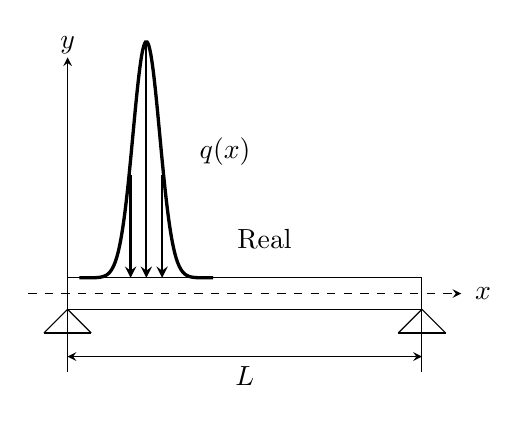
\begin{tikzpicture}
	\def\A{0.5*\ymax} % amplitude
    \def\T{0.1*\xmax} % width
	
	\node (A) at (1, 0.2) {};

    \draw[very thick,smooth,samples=\N,variable=\x,domain=-0.5*\xmax:0.5*\xmax, shift=(A)]
    plot(\x,{\A*exp(-(\x/(\T))^2/2)});

	\draw [-stealth, dashed] (-0.5, 0) -- (5, 0) node [near end, pos=1.05] {$x$};
	\draw [-stealth] (0, 0) -- (0, 3) node [near end, pos=1.05] {$y$};
	\draw (0, -0.2) rectangle (4.5, 0.2);

	\draw (0, -0.2) -- (-0.3, -0.5);
	\draw (0, -0.2) -- (0.3, -0.5);
	\draw (-0.3, -0.5) -- (0.3, -0.5);

	\draw (4.5, -0.2) -- (4.2, -0.5);
	\draw (4.5, -0.2) -- (4.8, -0.5);
	\draw (4.2, -0.5) -- (4.8, -0.5);

	\draw (0, 0) -- (0, -1);
	\draw (4.5, 0) -- (4.5, -1);

	\draw [>=stealth, <->] (0, -0.8) -- (4.5, -0.8) node [midway, below] {$L$};

	\draw [-stealth, thick] (0.8, 1.5) -- (0.8, 0.2);
	\draw [-stealth, thick] (1, 3.2) -- (1, 0.2);
	\draw [-stealth, thick] (1.2, 1.5) -- (1.2, 0.2);

	\node at (2, 1.8) {$q (x)$};
	\node at (2.5, 0.7) {Real};
	
\end{tikzpicture}
\end{document}